%% 
%% Copyright 2007-2020 Elsevier Ltd
%% 
%% This file is part of the 'Elsarticle Bundle'.
%% ---------------------------------------------
%% 
%% It may be distributed under the conditions of the LaTeX Project Public
%% License, either version 1.2 of this license or (at your option) any
%% later version.  The latest version of this license is in
%%    http://www.latex-project.org/lppl.txt
%% and version 1.2 or later is part of all distributions of LaTeX
%% version 1999/12/01 or later.
%% 
%% The list of all files belonging to the 'Elsarticle Bundle' is
%% given in the file `manifest.txt'.
%% 

%% Template article for Elsevier's document class `elsarticle'
%% with numbered style bibliographic references
%% SP 2008/03/01
%%
%% 
%%
%% $Id: elsarticle-template-num.tex 190 2020-11-23 11:12:32Z rishi $
%%
%%
\documentclass[preprint,12pt]{elsarticle}

%% Use the option review to obtain double line spacing
%% \documentclass[authoryear,preprint,review,12pt]{elsarticle}

%% Use the options 1p,twocolumn; 3p; 3p,twocolumn; 5p; or 5p,twocolumn
%% for a journal layout:
%% \documentclass[final,1p,times]{elsarticle}
%% \documentclass[final,1p,times,twocolumn]{elsarticle}
%% \documentclass[final,3p,times]{elsarticle}
%% \documentclass[final,3p,times,twocolumn]{elsarticle}
%% \documentclass[final,5p,times]{elsarticle}
%% \documentclass[final,5p,times,twocolumn]{elsarticle}

%% For including figures, graphicx.sty has been loaded in
%% elsarticle.cls. If you prefer to use the old commands
%% please give \usepackage{epsfig}

%% The amssymb package provides various useful mathematical symbols
\usepackage{amssymb}
\usepackage{multirow}
\usepackage{lineno}
\usepackage[colorlinks,citecolor=black,linkcolor=black,urlcolor=black,bookmarks,bookmarksnumbered]{hyperref}
%% The amsthm package provides extended theorem environments
\usepackage{amsthm}
\usepackage{amsmath}

%% The lineno packages adds line numbers. Start line numbering with
%% \begin{linenumbers}, end it with \end{linenumbers}. Or switch it on
%% for the whole article with \linenumbers.
%% \usepackage{lineno}

\journal{Energy}

\begin{document}

\begin{frontmatter}

%% Title, authors and addresses

%% use the tnoteref command within \title for footnotes;
%% use the tnotetext command for theassociated footnote;
%% use the fnref command within \author or \address for footnotes;
%% use the fntext command for theassociated footnote;
%% use the corref command within \author for corresponding author footnotes;
%% use the cortext command for theassociated footnote;
%% use the ead command for the email address,
%% and the form \ead[url] for the home page:
%% \title{Title\tnoteref{label1}}
%% \tnotetext[label1]{}
%% \author{Name\corref{cor1}\fnref{label2}}
%% \ead{email address}
%% \ead[url]{home page}
%% \fntext[label2]{}
%% \cortext[cor1]{}
%% \affiliation{organization={},
%%             addressline={},
%%             city={},
%%             postcode={},
%%             state={},
%%             country={}}
%% \fntext[label3]{}

\title{Self-tunable approximated explicit MPC: Heat exchanger implementation}
%\title{Self-tunable approximated explicit MPC: Implementation on a heat exchanger with a non-symmetric behavior}

%% use optional labels to link authors explicitly to addresses:
%% \author[label1,label2]{}
%% \affiliation[label1]{organization={},
%%             addressline={},
%%             city={},
%%             postcode={},
%%             state={},
%%             country={}}
%%
%% \affiliation[label2]{organization={},
%%             addressline={},
%%             city={},
%%             postcode={},
%%             state={},
%%             country={}}

\author{Lenka Galčíková}
\author{Juraj Oravec}
\author{Petronela Belková}

\affiliation{organization={Slovak University of Technology in Bratislava, Faculty of Chemical and Food Technology, Institute of Information Engineering, Automation, and Mathematics,},%Department and Organization
            addressline={Radlinského 9}, 
            city={Bratislava},
            postcode={81237}, 
%            state={Slovakia},
            country={Slovakia}
}

\begin{abstract}
max 250 words!

\end{abstract}

%%Graphical abstract
\begin{graphicalabstract}
%\includegraphics{grabs}
\end{graphicalabstract}

%%Research highlights
\begin{highlights}
\item Research highlight 1
\item Research highlight 2
\end{highlights}

\begin{keyword}
%% keywords here, in the form: keyword \sep keyword

%% PACS codes here, in the form: \PACS code \sep code

%% MSC codes here, in the form: \MSC code \sep code
%% or \MSC[2008] code \sep code (2000 is the default)

\end{keyword}

\end{frontmatter}

%% \linenumbers

%% main text
\section{Introduction}
\label{sec:introduction}


\section{Preliminaries}
\label{sec:preliminaries}

\subsection{Explicit model predictive control}
\label{sec:eMPC}
TODO: remark, ze sme si vedomi aj delta-u formulacie, ale vedie na zlozitejsie eMPC

\subsection{Tunable explicit model predictive control}
\label{sec:tunable}

\subsection{Self-tunable explicit model predictive control}
\label{sec:self_tunable}


\section{Methodology}
\label{sec:methodology}

\subsection{Self-tunable technique for systems with asymmetric behavior}
\label{sec:self_tunable_new}

TODO: spomenut, ze to je vhodne celkovo aj pre klasicke online MPC

\section{Results and discussion}
\label{sec:results}

In this section, the results of the proposed tuning method are presented. The plant on which the control was implemented is a laboratory liquid-to-liquid plate heat exchanger Armfield Process Plant Trainer PCT23~\cite{pct23}, see Fig.~\ref{fig:HE}. The cold feed as well as heating medium are transported to the heat exchanger by two peristaltic pumps. The flow rate of the feed is constant, while the aim is to track the reference value of its temperature. Therefore, the controlled variable is the feed temperature $T$ at the outlet of the heat exchanger and the manipulated variable is the voltage $U$ corresponding to the power of the heating medium pump. The voltage is set in percentage, while it is constrained from 20\% to 100\%. As the heat exchange is a nonlinear and non-symmetric process~\cite{Liptak}, this heat exchanger represents a suitable candidate for the presented controller tuning strategy.  

The matrices of the linear state-space model of the plant, discretized with sampling time $T_\mathrm{s}$ = 1\,s, are

\begin{subequations}
	\label{eq:model_A_B} 
	\begin{eqnarray}
		A&=&\begin{bmatrix}
			0.839
		\end{bmatrix}, \\
		B&=&\begin{bmatrix}
			0.039
		\end{bmatrix}, \\
		C&=&\begin{bmatrix}
			1
		\end{bmatrix}, \\
		D&=&\begin{bmatrix}
			0
		\end{bmatrix}.
		\end{eqnarray}
\end{subequations}

The constraints are considered in the terms of manipulated variable, i.e.

\begin{eqnarray}
\label{eq:u_const}
	-15\% \le u \le 65\%.
\end{eqnarray}

Note, the variable $u$ represents the manipulated variable in the deviation form. The values of feed temperature and voltage of the heating medium pump corresponding to zero steady state are respectively $T^\mathrm{s}$~=~35 $^{\circ}\mathrm{C}$ and $U^\mathrm{s}$~=~35\%.

The penalty matrices of the problem TODO:ref were systematically tuned and the corresponding control was implemented on the laboratory heat exchanger for every MPC setup. The aim was to determine, which penalty matrix will be the tuned one. Based on observations, the most significant effect on the control trajectories had tuning the penalty matrix $Q_\mathrm{y}$, while still preserving a satisfactory control performance, i.e., without steady-state control error and significant oscillations around the setpoint. The boundary values of matrix $Q_\mathrm{y}$ were tuned as $Q_\mathrm{y, L}$ = 100 and $Q_\mathrm{y, U}$ = 1000. The built-in integrator was penalized with $Q_\mathrm{x2}$ = 1 and the manipulated variable with $R$ = 10. The prediction horizon $N$ was 20 steps long. The control results for both control setups are compared in Fig.~\ref{fig:CV_boundaries} for the controlled variable, and in Fig.~\ref{fig:MV_boundaries} for the manipulated variable.
    

\begin{figure}
	\begin{center}
		\includegraphics[width=0.8\textwidth]{images/HE}
		\caption[Heat exchanger Armfield Process Plant Trainer PCT23]{Laboratory heat exchanger Armfield Process Plant Trainer PCT23: feed pump\,(1), heating medium pump\,(2), feed tanks\,(3), heater for heating medium\,(4), heat exchanger\,(5).}
		\label{fig:HE}
	\end{center}
\end{figure}

\begin{figure}
	\begin{center}
		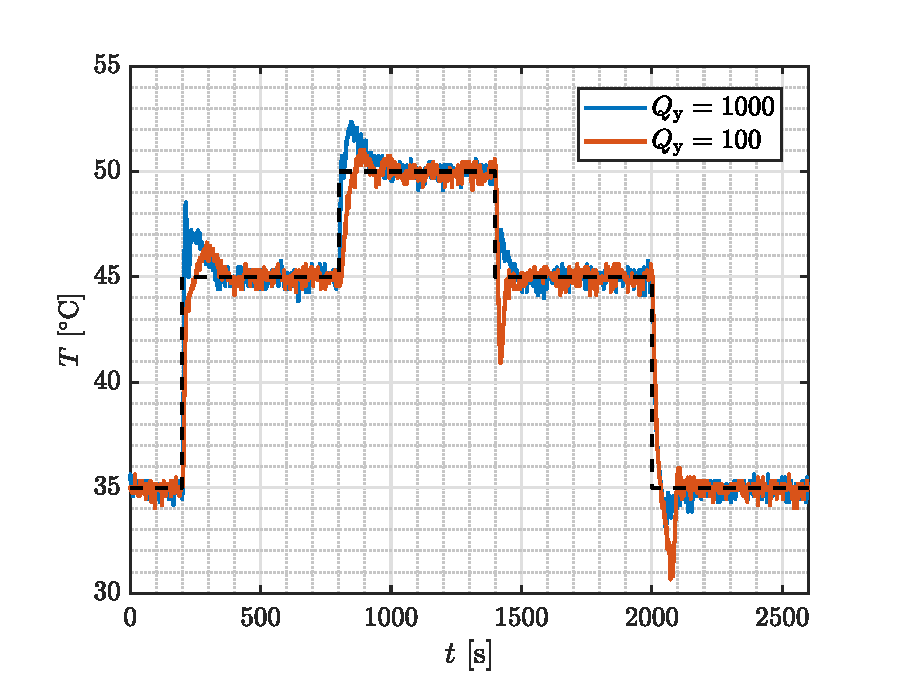
\includegraphics[width=0.8\textwidth]{images/CV_boundaries}
		\caption{Controlled variable trajectory for two boundary controllers. The solid lines represent the controlled temperature and the dashed line represents the reference value.}
		\label{fig:CV_boundaries}
	\end{center}
\end{figure}

The trajectories in Fig.~\ref{fig:CV_boundaries} show the non-symmetric nature of controlling the process of heat exchange mainly when observing the overshoots and undershoots. When applying the control associated with the lower bound $Q_\mathrm{y, L}$, significant undershoots are present when tracking the reference downwards, i.e., when the reference change is negative. On the contrary, when implementing the controller associated with $Q_\mathrm{y, U}$, the undershoots are negligible, but significant overshoots can be seen when tracking the reference upwards.

These observations form the base for the strategy of self-tuning the penalty matrix $Q_\mathrm{y}$. The strategy follows the ideas summarized in Section~\ref{sec:self_tunable_new}.

\begin{figure}
	\begin{center}
		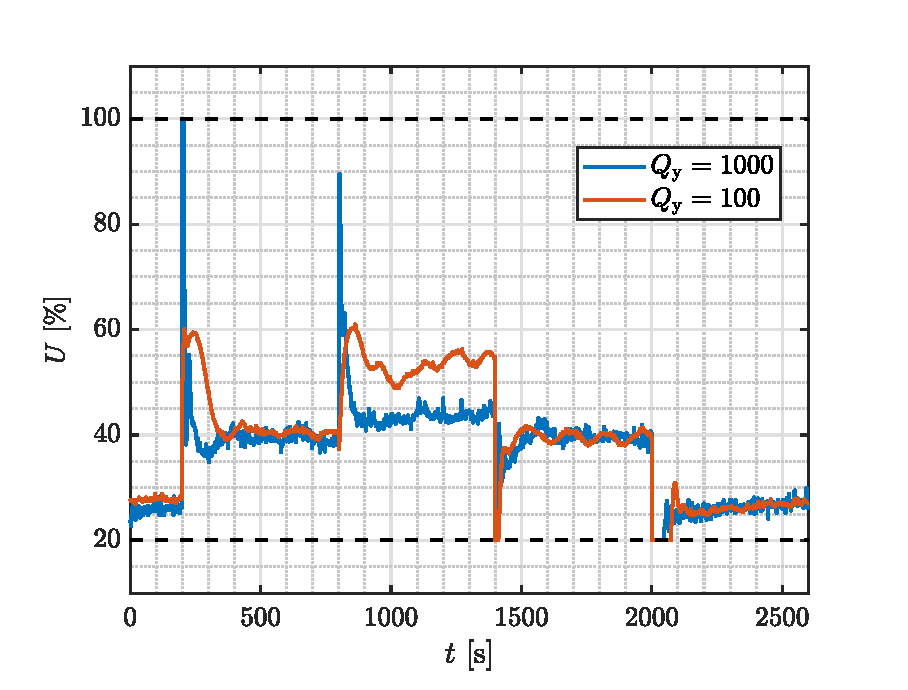
\includegraphics[width=0.8\textwidth]{images/MV_boundaries}
		\caption{Manipulated variable trajectory for two boundary controllers. The solid lines represent the voltage and the dashed lines represent the constraints.}
		\label{fig:MV_boundaries}
	\end{center}
\end{figure}

\begin{figure}
	\begin{center}
		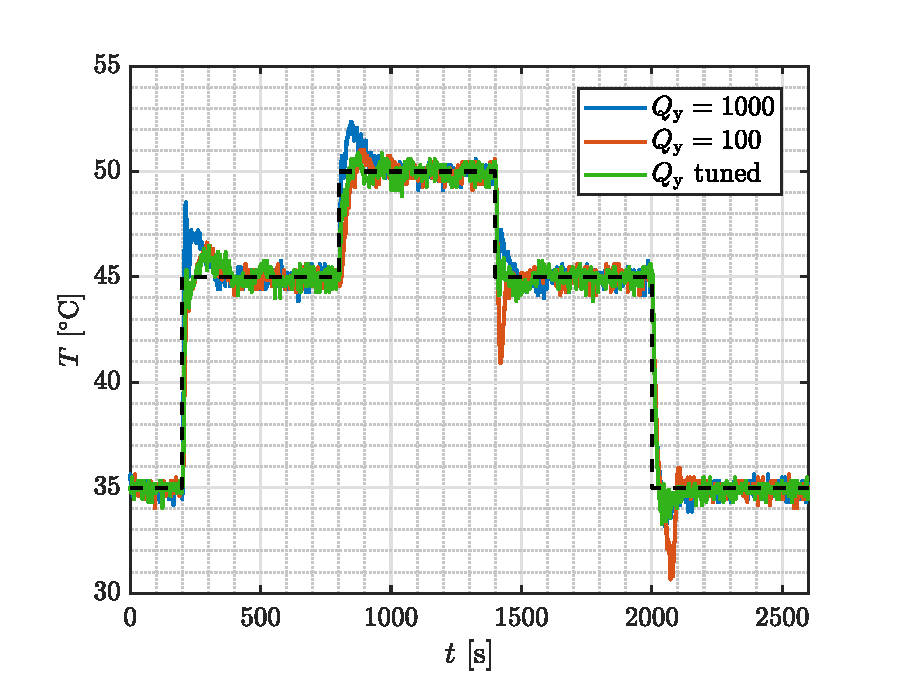
\includegraphics[width=0.8\textwidth]{images/CV}
		\caption{Controlled variable trajectory for two boundary controllers and the tuned one. The solid lines represent the controlled temperature and the dashed line represents the reference value.}
		\label{fig:CV}
	\end{center}
\end{figure}

\begin{figure}
	\begin{center}
		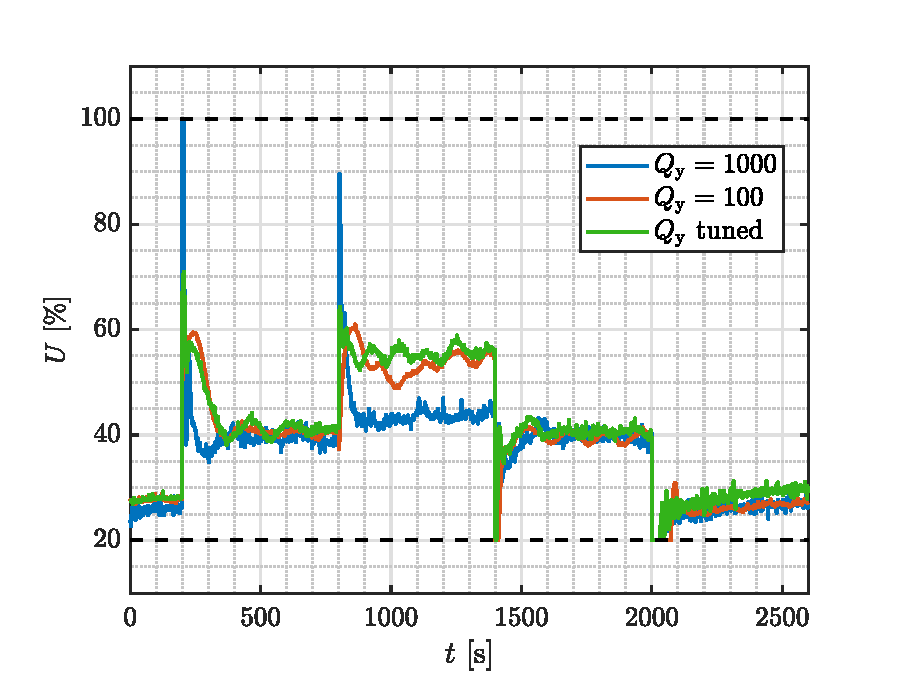
\includegraphics[width=0.8\textwidth]{images/MV}
		\caption{Manipulated variable trajectory for two boundary controllers and the tuned one. The solid lines represent the voltage and the dashed lines represent the constraints.}
		\label{fig:MV}
	\end{center}
\end{figure}

\begin{table}[h!]
	\begin{center}
		\caption{Control performance criteria.}
		\label{tab:control_performance}
		\begin{tabular}{c|c|c|c|c|c} 
			Reference step change & $Q_\mathrm{y}$ & ISE [$^{\circ}\mathrm{C}^2$\,s] & $\sigma_{\mathrm{max}}$\,[\%] & $t_{\epsilon}$\,[s] & $V$\,[l] \\
			\hline
			\multirow{2}{*}{1} & 1000 & 714 & 33.50 & 16.5 & \textbf{2.12} \\
			    & 100 & 867 & 16.65 & 12.5 & 2.36 \\ 
			    & tuned & \textbf{678} & \textbf{15.19} & \textbf{9.5} & 2.38 \\ 
			\hline
			\multirow{2}{*}{2} & 1000 & 365 & 47.20 & \textbf{5} & \textbf{2.49} \\
			    & 100 & 606 & 23.25 & 26.5 & 3.19 \\ 
			    & tuned & \textbf{248} & \textbf{19.13} & 9.5 & 3.35 \\ 
			\hline
		    \multirow{2}{*}{3} & 1000 & 245 & \textbf{18.92} & \textbf{6.5} & \textbf{2.00} \\
				& 100 & 398 & 79.64 & 31 & \textbf{2.00} \\ 
				& tuned & \textbf{186} & 24.59 & \textbf{6.5} & 2.10 \\ 
			\hline
			\multirow{2}{*}{4} & 1000 & 1024 & 18.43 & 22.5 & 0.94 \\
				& 100 & 1402 & 41.87 & 90 & \textbf{0.93} \\ 
				& tuned & \textbf{967} & \textbf{16.49} & \textbf{18.5} & 1.10  
		\end{tabular}
	\end{center}
\end{table}

\section{Conclusion}
\label{sec:conclusion}


%% The Appendices part is started with the command \appendix;
%% appendix sections are then done as normal sections
%% \appendix

%% \section{}
%% \label{}

%% If you have bibdatabase file and want bibtex to generate the
%% bibitems, please use
%%

\bibliographystyle{elsarticle-num} 
\bibliography{references}

%% else use the following coding to input the bibitems directly in the
%% TeX file.

%\begin{thebibliography}{00}
%
%%% \bibitem{label}
%%% Text of bibliographic item
%
%\bibitem{}
%
%\end{thebibliography}

\end{document}
\endinput
%%
%% End of file `elsarticle-template-num.tex'.
